\documentclass[%
	final, %
	% draft, % Grafische Elemente durch graue Boxen ersetzen (beschleunigt Kompilieren)
	% 8pt, % Zu klein, erfordert Paket extsize
	% 9pt, % Zu klein, erfordert Paket extsize
	% 10pt, % für Folien mit sehr viel Text
	11pt, % Standardschriftgröße
	% 12pt, % etwas größer und daher besser zu lesen
	% 14pt, % deutlich größer, erfordert Paket extsize
	% 17pt, % PowerPoint Standardschriftgröße, erfordert Paket extsize
	% 20pt, % sehr groß, erfordert Paket extsize
	% trans,% Zum Erstellen von Overhead Folien
	% handout, % Erstellen eines Handouts
	% article,% Erstellen eines Artikels
 	% compress, % Die Navigation in der Kopfzeile wird komprimiert dargestellt
	t, % Place text of slides at the (vertical) top of the slides
	% c, % Place text of slides at the (vertical) center of the slides
	% color={}, % list of options for color
	xcolor={table,dvipsnames}, % Optionen für xcolor übergeben
	% hyperref={}, % list of options for hyperref
	% envcountsect, % Causes theorems, definitions, and so on to be numbered locally to each section.
	% notheorems, % Switches off the definition of default blocks like theorem
	% noamsthm, % Does not load amsthm and also not amsmath
	% ucs, % lädt ucs Paket
	% utf8, % lädt utf8x Paket von ucs (utf8 enconding)
	% dvips, % erzwingt das Laden des dvips Treibers - idR nicht nötig!
	% usepdftitle=false, % Suppresses the automatic generation of title and author entries in the pdf document information.
	% ignorenonframetext, % suppresses content created for the article mode ??
	show notes, % enables Notes
	% leqno,
	% fleqn,
]{beamer}[2007/03/11] % Minimum necessary version due to severe bugs in version 3.06 !!!



% ~~~~~~~~~~~~~~~~~~~~~~~~~~~~~~~~~~~~~~~~~~~~~~~~~~~~~~~~~~~~~~~~~~~~~~~~
% Fonts Fonts Fonts
% ~~~~~~~~~~~~~~~~~~~~~~~~~~~~~~~~~~~~~~~~~~~~~~~~~~~~~~~~~~~~~~~~~~~~~~~~
\usepackage[T1]{fontenc} % T1 Schrift Encoding
\usepackage{textcomp}	 % additional symbols (Text Companion font extension)


% \usepackage{lmodern}               %% --- Latin Modern
\usepackage{mathptmx}              %% --- Times mit Matheschriften
% \usepackage{mathpazo}              %% --- Palantino
% \usepackage{charter}               %% --- Charter
% \usepackage{bookman}               %% Bookman (lädt Avant Garde !!)
% \usepackage{newcent}               %% New Century Schoolbook (lädt Avant Garde !!)

% \usepackage{bera}
\usepackage[scaled=.90]{helvet}    %% --- Helvetica (Arial)
% \usepackage{cmbright}              %% --- CM-Bright (eigntlich eine Familie)
% \usepackage{tpslifonts}            %% --- (Font for Slides)
% \usepackage{avant}      	          %% --- Avantgard
%
\usepackage{courier}               %% --- Courier
%\usepackage[scaled=0.9]{luximono}  	 %% --- Luxi Mono


%%% ===== Sans Serif (kommerzielle Schriften) ============================

% \usepackage[scaled=0.90]{frutiger}  %% --- Adobe Frutiger
% \usepackage[scaled=0.94]{futura}    %% --- Adobe Futura (=Linotype FuturaLT) : Sans Serif
% \usepackage{gillsans}               %% --- Adobe Gill Sans : Sans Serif
% \renewcommand{\sfdefault}{pmy}      %% -- Adobe Myriad  : Sans Serif
% \usepackage[scaled]{asyntax}        %% --- Syntax : sans serif font
% \usepackage[medium]{optima}         %% --- Adobe Optima : Semi Sans Serif
% \renewcommand{\sfdefault}{lo9}      %% --- Linotype ITC Officina Sans

%% ===== Serifen (kommerzielle Schriften ) ================================

% \renewcommand{\rmdefault}{pasx}     %% --- Adobe Aldus
% \usepackage[scaled=1.05]{xagaramon} %% --- Adobe Garamond
% \renewcommand{\rmdefault}{pegx}     %% --- Adobe Stempel Garamond
% \renewcommand{\rmdefault}{pml}      %% --- Adobe Melior
% \renewcommand{\rmdefault}{pmnx}     %% --- Adobe Minion
% \renewcommand{\rmdefault}{psbx}     %% --- Adobe Sabon
% \renewcommand{\rmdefault}{lch}      %% --- Linotype ITC Charter
% \renewcommand{\rmdefault}{lmd}      %% --- Linotype Meridien

% *** Sprache *****************************
\usepackage[ngerman]{babel}
\usepackage[utf8]{inputenc}
%------------------------------------------


%%% Doc: ftp://tug.ctan.org/pub/tex-archive/macros/latex/required/graphics/grfguide.pdf
% Bilder
\usepackage[%
   %final,
   %draft % do not include images (faster)
]{graphicx}



%%% Emulationspakete
% \usepackage{beamerprosper}
% \usepackage{beamerseminar}
% \usepackage{beamerfoils}
% \usepackage{beamertexpower}


%%% 4.6.2    Printing the Handout
% \usepackage{pgfpages}
% \pgfpagelayout{resize}[a4paper,border shrink=5mm,landscape]
%     This says “Resize all pages to landscape A4 pages, no what their original size was, but shrink the pages
% by 5mm, so that there is a bit of a border around everything.” Naturally, instead of a4paper you can also use
% letterpaper or any of the other standard paper sizes. For further options and details see the documentation
% of pgfpages.
% \pgfpagelayout{2 on 1}[a4paper,border shrink=5mm]


% \usepackage{multimedia}
%     A stand-alone package that implements several commands for including external animation and sound
%     files in a pdf document. The package can be used together with both dvips plus ps2pdf and pdflatex,
%     though the special sound support is available only in pdflatex.



%% sonstige Pakete ========================
%
% \usepackage{enumitem}
% \usepackage{units}
% \usepackage{pifont}
% \usepackage{subscript}
% -----------------------------------------

\usepackage{tabularx}   % Erweiterte Tabellen Optionen
\usepackage{booktabs}
\usepackage{multicol}







% *****************************************
% >>> Themes <<<<<<<<<<<<<<<<<<<<<<<<<<<<<<
% *****************************************

% \usetheme[<options>]{<name list>} 		Installs the presentation theme named <name>.
% \usecolortheme[<options>]{<name list>} Same as \usetheme, only for color themes.
% \usefonttheme[<options>]{<name>} 		Same as \usetheme, only for font themes.
% \useinnertheme[<options>]{<name>}		Same as \usetheme, only for inner themes.
% \useoutertheme[<options>]{<name>}		Same as \usetheme, only for outer themes.

% *****************************************
% >>> Themes ohne Navigation
% *****************************************
% \usetheme{default}
% -------------------------------
% \usetheme[]{Bergen}
% -------------------------------
% \usetheme[%
% 	secheader % section im Header
% ]{Boadilla}
% -------------------------------
% % Wie das Boadilla theme, mit kraeftigeren Farben
% % und unveraenderten Icons
% \usetheme[%
% 	secheader % section im Header
% ]{Madrid}
% -------------------------------
% \usetheme{Pittsburgh}
% -------------------------------
% \usetheme[]{Rochester}


% *****************************************
% >>> Themes mit Navigation (Baumstruktur)
% *****************************************
% \usetheme{Antibes}      % flach
% -------------------------------
% \usetheme{JuanLesPins}  % 3D, Schatten
% -------------------------------
% \usetheme{Montpellier}    % flach, wenig Farben


% *****************************************
% >>> Themes mit Navigation (Sidebar)
% *****************************************
% % flach, starke Farben
% \usetheme[%
%  	left, % sidebar links
% % 	right, % sidebar rechts
% % 	hideallsubsections, % nur sections werden angezeigt
% % 	hideothersubsections, % nur subsections der aktuellen section werden angezeigt
% ]{Berkeley}
% -------------------------------
% % wie Berkeley, 3D, starke Farben
% \usetheme[%
%  	left, % sidebar links
% % 	right, % sidebar rechts
% % 	hideallsubsections, % nur sections werden angezeigt
% % 	hideothersubsections, % nur subsections der aktuellen section werden angezeigt
% ]{PaloAlto}
% -------------------------------
% % flach, schwache Farben
% \usetheme[%
%  	left, % sidebar links
% % 	right, % sidebar rechts
% % 	hideallsubsections, % nur sections werden angezeigt
% % 	hideothersubsections, % nur subsections der aktuellen section werden angezeigt
% ]{Goettingen}
% -------------------------------
% % wie Goettingen, flach, starke Farben
% \usetheme[%
%  	left, % sidebar links
% % 	right, % sidebar rechts
% % 	hideallsubsections, % nur sections werden angezeigt
% % 	hideothersubsections, % nur subsections der aktuellen section werden angezeigt
% ]{Marburg}
% -------------------------------
% flach, schwache Farben
% \usetheme[%
% % 	hideallsubsections, % nur sections werden angezeigt
% % 	hideothersubsections, % nur subsections der aktuellen section werden angezeigt
% ]{Hannover}


% *****************************************
% >>> Themes mit Navigation (Mini Frame Navigation)
% *****************************************
% % starke Farben, flach
% \usetheme[
% % 	compress, % Navigation in einer Zeile
% ]{Berlin}
% -------------------------------
% % wie Berlin, runde Kanten, starke Farben, flach
 \usetheme[
 	compress, % Navigation in einer Zeile
 ]{Ilmenau}
% -------------------------------
% % wie Berlin, starke Farben, flach
% \usetheme[
% 	compress, % Navigation in einer Zeile
% ]{Dresden}
% -------------------------------
% % starke Farben, 3D
% \usetheme{Darmstadt}
% -------------------------------
% % wie Darmstadt, ohne subsections
% \usetheme{Frankfurt}
% -------------------------------
% % flach, schwache Farben
% \usetheme{Singapore}
% -------------------------------
% % flach, horiz. Linien
% \usetheme{Szeged}


% *****************************************
% >>> Themes mit Navigation (Section and Subsection Tables)
% *****************************************
% % flach, rund, starke Farben
% \usetheme{Copenhagen}
% -------------------------------
% % flach, eckig, starke Farben
% \usetheme{Luebeck}
% -------------------------------
% % flach, starke Farben
% \usetheme{Malmoe}
% -------------------------------
% 3D, starke Farben
%\usetheme{Warsaw}


% *****************************************
% >>>> 15.1    Inner Themes
% *****************************************
% An inner theme installs templates that dictate how the following elements are typeset:
%    - Title and part pages.
%    - Itemize environments.
%    - Enumerate environments.
%    - Description environments.
%    - Block environments.
%    - Theorem and proof environments.
%    - Figures and tables.
%    - Footnotes.
%    - Bibliography entries.


% >>>  Itemize Bullets
% -------------------------------
% \useinnertheme{default} % Zahlen
% -------------------------------
% \useinnertheme{circles} % Kreise
% -------------------------------
\useinnertheme{rectangles} % Vierecke
% -------------------------------
%\useinnertheme[%
%	shadow % mit Schatten
% ]{rounded} % 3D Kugeln
% -------------------------------
% \useinnertheme{inmargin} % Bullts im Margin


% *****************************************
% >>>> 15.2    Outer Themes
% *****************************************
% An outer theme dictates (roughly) the overall layout of frames. It specifies where any navigational elements
% should go (like a mini table of contents or navigational mini frames) and what they should look like. Typically,
% an outer theme specifies how the following elements are rendered:
%    - The head- and footline.
%    - The sidebars.
%    - The logo.
%    - The frame title.

% \useoutertheme{default}
% -------------------------------
% \useoutertheme{infolines}
% -------------------------------
% \useoutertheme[%
% 	footline=empty, % suppressed the footline (default).
% % 	footline=authorinstitute, %shows the author's name and the institute in the footline.
% % 	footline=authortitle, % shows the author's name and the title in the footline.
% % 	footline=institutetitle, % shows the institute and the title in the footline.
% % 	footline=authorinstitutetitle, % shows the author's name, the institute, and the title in the footline.

% ]{miniframes}
% -------------------------------
% \useoutertheme[%
% % 	subsection= true,  % or false shows or suppresses line showing the subsection in the headline.
% ]{smoothbars}
% -------------------------------
% \useoutertheme[%
%  	left, % sidebar links
% % 	right, % sidebar rechts
% % 	hideallsubsections, % nur sections werden angezeigt
% % 	hideothersubsections, % nur subsections der aktuellen section werden angezeigt
% ]{sidebar}
% -------------------------------
% % This theme installs a headline in which, on the left, the sections of the talk are shown and, on the right,
% % the subsections of the current section. If the class option compress has been given, the sections and
% % subsections will be put in one line; normally there is one line per section or subsection.
% \useoutertheme{split}
% The colors are taken from palette primary and palette fourth.
% -------------------------------
% % This layout theme extends the split theme by putting a horizontal shading behind the frame title and
% % adding a little 'shadow' at the bottom of the headline.
% \useoutertheme{shadow}
% -------------------------------
% \useoutertheme[
% % 	hooks, % Einruecken der Abschnittsueberschriften in der Kopfzeile
% ]{tree}
% -------------------------------
% wie tree, ohne die Linien
% \useoutertheme{smoothtree}


% *****************************************
% >>>> 16.1    Color Themes
% *****************************************
% \usecolortheme{default}
% \usecolortheme{structure}
% \usecolortheme{sidebartab}

% *****************************************
% >>>> 16.1.2    Complete Color Themes
% A 'complete' color theme is a color theme that completely specifies all colors for all parts of a frame. It
% installs specific colors and does not derive the colors from, say, the structure beamer-color. Complete
% color themes happen to have names of flying animals.

% -------------------------------
% \usecolortheme{default}
% -------------------------------
\usecolortheme[%
% 	named=red,
% 	named=blue,
% 	named=green,
% 	named=orange,
% 	named=gray,
 	named=NavyBlue,
%  named=RoyalBlue,
%  named=MidnightBlue,
%  named=CadetBlue,
]{structure}
% Farben aus dvipsnam.def: (Option 'dvipsnames' fuer xcolor muss geladen sein!)
% http://www.math.utu.fi/opetusohj/latex/doc/palette.pdf
% GreenYellow, Yellow, Goldenrod, Dandelion, Apricot, Peach, Melon, YellowOrange, Orange, BurntOrange, Bittersweet, RedOrange, Mahogany, Maroon, BrickRed, Red, OrangeRed, RubineRed, WildStrawberry, Salmon, CarnationPink, Magenta, VioletRed, Rhodamine, Mulberry, RedViolet, Fuchsia, Lavender, , Thistle, Orchid, DarkOrchid, Purple, Plum, Violet, RoyalPurple, BlueViolet, Periwinkle, CadetBlue, CornflowerBlue, MidnightBlue, NavyBlue, RoyalBlue, Blue, Cerulean, Cyan, ProcessBlue, , SkyBlue, Turquoise, TealBlue, Aquamarine, BlueGreen, Emerald, JungleGreen, SeaGreen, Greenv,  ForestGreen, PineGreen, LimeGreen, YellowGreen, SpringGreen, OliveGreen, RawSienna, Sepia, Brown, Tan, Gray, Black, White
% -------------------------------
% % blau-schwarz, Hintergrund: blau
% \usecolortheme[%
% %  	overlystylish
% ]{albatross}
% -------------------------------
% % blau-schwarz, Hintergrund: weiss
% \usecolortheme{lily}
% -------------------------------
% % blau-grau, , Hintergrund: grau
% \usecolortheme{beetle}
% -------------------------------
% % gelb-weiss, , Hintergrund: weiss
% \usecolortheme{crane}
% -------------------------------
% grau-grau (hell)
% \usecolortheme{dove}
% -------------------------------
% % grau-grau (dunkel)
% \usecolortheme{fly}
% -------------------------------
% % grau-grau-weiss (hell) mit Boxen
% \usecolortheme{seagull}
% -------------------------------
% % gelb-orange-grau
% \usecolortheme{wolverine}
% -------------------------------
% % grau
% \usecolortheme{beaver}

% *****************************************
% >>>> 16.1.3    Inner Color Themes
% Inner color themes only specify the colors of elements used in inner themes. Most noticably, they specify
% the colors used for blocks. They can be used together with other (color) themes. If they are used to change
% the inner colors installed by a presentation theme or another color theme, they should obviously be specified
% after the other theme has been loaded. Inner color themes happen to have fl�ower names.
% -------------------------------
% \usecolortheme{lily} % keine Boxen
% -------------------------------
% \usecolortheme{orchid} % Boxen mit starken Farben
% -------------------------------
% \usecolortheme{rose} % Boxen mit schwachen Farben

% *****************************************
% >>>> 16.1.4    Outer Color Themes
% An outer color theme changes the palette colors, on which the colors used in the headline, footline, and
% sidebar are based by default. Outer color themes normally do not change the color of inner elements, except
% possibly for titlelike. They have happen to sea-animal names.

% -------------------------------
% % Titel mit Farbe, starke Farben
% \usecolortheme{whale}
% -------------------------------
% % Titel mit Farbe, schwache Farben
% \usecolortheme{seahorse}
% -------------------------------
% % Titel ohne Farbe, starke Farben
% \usecolortheme{dolphin}

% *****************************************
% Detailierte Veraenderungen der Farben
% *****************************************
% \setbeamercolor*{author in head/foot}{parent=palette tertiary}
% \setbeamercolor*{title in head/foot}{parent=palette secondary}
% \setbeamercolor*{date in head/foot}{parent=palette primary}
% \setbeamercolor*{section in head/foot}{parent=palette secondary} %tertiary
% \setbeamercolor*{subsection in head/foot}{parent=palette primary}
% Elemente deren Farbe veraendert werden kann
% \setbeamercolor{normal text}{fg=black}
% \setbeamercolor*{example text}
% \setbeamercolor*{titlelike}
% \setbeamercolor*{separation line}
% \setbeamercolor*{upper separation line head}
% \setbeamercolor*{separation line}
% \setbeamercolor*{middle separation line head}
% \setbeamercolor*{separation line}
% \setbeamercolor*{lower separation line head}
% \setbeamercolor*{upper separation line foot}
% \setbeamercolor*{middle separation line foot}
% \setbeamercolor*{lower separation line foot}
% -------------------------------
% \setbeamercolor*{math text}
% \setbeamercolor*{math text inlined}
% \setbeamercolor*{math text displayed}
% \setbeamercolor*{normal text in math text}
% -------------------------------
% Nutzung:
% \usebeamercolor[fg]{normal text}
% \setbeamercolor{normal text}{fg=black,bg=mylightgrey}
% -------------------------------
% Palette:
% \setbeamercolor{palette primary}
% \setbeamercolor{palette secondary}
% \setbeamercolor{palette tertiary}
% \setbeamercolor{palette quaternary}
% -------------------------------
% \setbeamercolor{palette sidebar primary}
% \setbeamercolor{palette sidebar secondary}
% \setbeamercolor{palette sidebar tertiary}
% \setbeamercolor{palette sidebar quaternary}




% *****************************************
% Transparenz Effekte
% *****************************************

\setbeamercovered{invisible} % is the default and causes covered text to 'completely disappear.
% \setbeamercovered{transparent} % Durchscheinen des Textes
% \setbeamercovered{dynamic} % Einblenden
% \setbeamercovered{highly dynamic} % Einblenden


% *****************************************
% >>>> 17.1 Font Themes
% *****************************************
% \usefonttheme{default}
% The default font theme installs a sans serif font for all text of the presentation. The default theme
% installs different font sizes for things like titles or head- and footlines, but does not use boldface or
% italics for 'hilighting.' To change some or all text to a serif font, use the serif theme.
% -------------------------------
% \usefonttheme{professionalfonts}
% This font theme does not really change any fonts. Rather, it suppresses certain internal replacements
% performed by beamer. If you use 'professional fonts' (fonts that you buy and that come with a
% complete set of every symbol in all modes), you do not want beamer to meddle with the fonts you use.
% -------------------------------
% \usefonttheme[%
% % 	stillsansserifmath, % mathematical text typeset using sans serif.
% % 	stillsansserifsmall, % will cause 'small' text to be still typeset using sans serif. This refers to
%  								% the text in the headline, footline, and sidebars. Using this options is often
%  								% advisable since small  text is often easier to read in sans serif.
% % 	stillsansseriflarge, %  Titel still   typeset using sans serif
% %  	onlymath, % typset math in serif but nothing else
% ]{serif}
% -------------------------------
% \usefonttheme[%
% % 	onlysmall, % headline, footline, and sidebars is changed
% % 	onlylarge, % main title, frame titles, and section
% ]{structurebold}
% -------------------------------
% \usefonttheme[%
% % 	onlysmall, % headline, footline, and sidebars is changed
% % 	onlylarge, % main title, frame titles, and section
% ]{structureitalicserif}
% -------------------------------
% \usefonttheme[%
% % 	onlysmall, % headline, footline, and sidebars is changed
% % 	onlylarge, % main title, frame titles, and section
% ]{structuresmallcapsserif}



% *****************************************
% >>>> Veraendern der Schrifteinstellung definierter Elemente
% *****************************************

% Beispiele
% \setbeamerfont{frametitle}{size=\large}
% \setbeamerfont{frametitle}{series=\bfseries}

% weitere Befehle
% size= size command sets the size attribute of the beamerfont.
% size*={ size in pt }{ baselineskip }
% shape= (\itshape, \slshape, \scshape, or \upshape)
% series= (command like \bfseries.)
% family= (command like \rmfamily or \sffamily).
% family*={ family name } (For example, the family name for Times happens to be ptm. )
% parent={ parent list } specifies a list of parent fonts.
%
% Example for parent
% \setbeamerfont{parent A}{size=\large}
% \setbeamerfont{parent B}{series=\bfseries}
% \setbeamerfont{child}{parent={parent A, parent B},size=\small}
%
% \usebeamerfont{child}
% This text is small and bold.

% *****************************************
% >>>> 15.3.2    Using Beamer's Templates
% *****************************************
% As a user of the beamer class you typically do not 'use' or 'invoke' templates yourself, directly. For
% example, the frame title template is automatically invoked by beamer somewhere deep inside the frame
% typesetting process. The same is true of most other templates. However, if, for whatever reason, you wish
% to invoke a template yourself, you can use the following command.
% \usebeamertemplate***{ element name }
% -------------------------------
%%% 7.2.1 The Headline and Footline
% \setbeamertemplate{headline} % Beamer-Template/-Color/-Font
% \setbeamertemplate{headline}
% {%
%   \begin{beamercolorbox}{section in head/foot}
%     \vskip2pt\insertnavigation{\paperwidth}\vskip2pt
%   \end{beamercolorbox}%
% }
% \setbeamertemplate{headline}[default] % The default is just an empty headline.
% \setbeamertemplate{headline}[infolines theme]
% \setbeamertemplate{headline}[miniframes theme]
% \setbeamertemplate{headline}[sidebar theme]
% \setbeamertemplate{headline}[smoothtree theme]
% \setbeamertemplate{headline}[smoothbars theme]
% \setbeamertemplate{headline}[tree]
% \setbeamertemplate{headline}[split theme]
% \setbeamertemplate{headline}[text line]{ text } % The headline is typeset with 'text'
% -------------------------------
% \setbeamertemplate{footline} % Beamer-Template/-Color/-Font
% \setbeamertemplate{footline}[default]
% \setbeamertemplate{footline}[infolines theme]
% \setbeamertemplate{footline}[miniframes theme]
% \setbeamertemplate{footline}[page number]
% \setbeamertemplate{footline}[frame number]
% \setbeamertemplate{footline}[split]
% \setbeamertemplate{footline}[text line]{ text }
% -------------------------------
%%% 7.2.2 The Sidebars
% -------------------------------
%%% 7.2.3 Navigation Bars (funktioniert nur mit miniframe Themes)
% \setbeamertemplate{mini frames}[default] % shows small circles as mini frames.
\setbeamertemplate{mini frames}[box] % shows small rectangles as mini frames.
% \setbeamertemplate{mini frames}[tick] % shows small vertical bars as mini frames.
% -------------------------------
%%% 7.2.4 The Navigation Symbols
%%% Beamer-Template/-Color/-Font navigation symbols
\setbeamertemplate{navigation symbols}{} % suppresses all navigation symbols:
% \setbeamertemplate{navigation symbols}[horizontal] % Organizes the navigation symbols horizontally.
% \setbeamertemplate{navigation symbols}[vertical] % Organizes the navigation symbols vertically.
% \setbeamertemplate{navigation symbols}[only frame symbol] % Shows only the navigational symbol for navigating frames.
% -------------------------------
%%% 7.2.5 The Logo
% \setbeamertemplate{logo} % Beamer-Template/-Color/-Font
% -------------------------------
%%% 7.2.6 The Frame Title
% \setbeamertemplate{frametitle} % Beamer-Template/-Color/-Font
% \setbeamertemplate{frametitle}[default][left] % left, center, right
% \setbeamertemplate{frametitle}[shadow theme]
% \setbeamertemplate{frametitle}[sidebar theme]
% \setbeamertemplate{frametitle}[smoothbars theme]
% \setbeamertemplate{frametitle}[smoothtree theme]
% -------------------------------
%%% 7.2.7 The Background
% \setbeamertemplate{background canvas} % Beamer-Template/-Color/-Font
% \setbeamertemplate{background canvas}[default]
% \setbeamertemplate{background canvas}[vertical shading][ color options ] installs a vertically shaded background.
%     - top= color specifies the color at the top of the page. By default, 25% of the foreground of
%       the beamer-color palette primary is used.
%     - bottom= color specifies the color at the bottom of the page. By default, the background of
%       normal text at the moment of invocation of this command is used.
%     - middle= color specifies the color for the middle of the page. Thus, if this option is given, the
%       shading changes from the bottom color to this color and then to the top color.
%     - midpoint= factor specifies at which point of the page the middle color is used. A factor of 0
%       is the bottom of the page, a factor of 1 is the top. The default, which is 0.5 is in the middle.
% \setbeamertemplate{background} % Beamer-Template/-Color/-Font
% \setbeamertemplate{background}[default] % is empty.
% \setbeamertemplate{background}[grid][step=1cm] % places a grid on the background.
%     - step= dimension specifies the distance between grid lines. The default is 0.5cm.
%     - color= color specifies the color of the grid lines. The default is 10% foreground.
% -------------------------------
%%% 7.3 Margin Sizes
\setbeamersize{text margin left=2em,text margin right=2em}
% \setbeamersize{sidebar width left=2cm}
%         - text margin left= TEX dimension sets a new left margin. This excludes the left sidebar. Thus,
%           it is the distance between the right edge of the left sidebar and the left edge of the text.
%         - text margin right= TEX dimension sets a new right margin.
%         - sidebar width left= TEX dimension sets the size of the left sidebar. Currently, this command
%           should be given before a shading is installed for the sidebar canvas.
%         - sidebar width right= TEX dimension sets the size of the right sidebar.
%         - description width= TEX dimension sets the default width of description labels, see Section 11.1.
%         - description width of= text sets the default width of description labels to the width of the
%             text , see Section 11.1.
%         - mini frame size= TEX dimension sets the size of mini frames in a navigation bar. When two
%           mini frame icons are shown alongside each other, their left end points are TEX dimension far
%           apart.
%         - mini frame offset= TEX dimension set an additional vertical offset that is added to the mini
%           frame size when arranging mini frames vertically.
% -------------------------------
%%% 9.1 Adding a Title Page
% \setbeamersize{title page} % Beamer-Template/-Color/-Font
%    This template is invoked when the \titlepage command is used.
%    The following commands are useful for this template:
%     -  \insertauthor inserts a version of the author's name that is useful for the title page.
%     -  \insertdate inserts the date.
%     -  \insertinstitute inserts the institute.
%     -  \inserttitle inserts a version of the document title that is useful for the title page.
%     -  \insertsubtitle inserts a version of the document title that is useful for the title page.
%     -  \inserttitlegraphic inserts the title graphic into a template.
% -------------------------------
%%% 9.2 Adding Sections and Subsections
% -------------------------------
%%% Parent Beamer-Template sections/subsections in toc
% This is a parent template, whose children are section in toc and subsection in toc.
% \setbeamertemplate{sections/subsections in toc}[default]
% \setbeamertemplate{sections/subsections in toc}[sections numbered]
% \setbeamertemplate{sections/subsections in toc}[subsections numbered]
% \setbeamertemplate{sections/subsections in toc}[circle]
\setbeamertemplate{sections/subsections in toc}[square]
% \setbeamertemplate{sections/subsections in toc}[ball]
% \setbeamertemplate{sections/subsections in toc}[ball unnumbered]
% -------------------------------
%%% 9.6 Adding a Bibliography
% -------------------------------
% \setbeamertemplate{bibliography item} % Beamer-Template/-Color/-Font
\setbeamertemplate{bibliography item}[default] %  little article icon as the reference
% \setbeamertemplate{bibliography item}[article] % Alias for the default.
% \setbeamertemplate{bibliography item}[book] % little book icon as the reference
% \setbeamertemplate{bibliography item}[triangle] % triangle as the reference
% \setbeamertemplate{bibliography item}[text] % reference text (like '[Dijkstra, 1982]')
% -------------------------------
%%% 10.1 Adding Hyperlinks and Buttons
% -------------------------------
%%% 11.1 Itemizations, Enumerations, and Descriptions
% \setbeamertemplate{items} % parent template of itemize items and enumerate items
% \setbeamertemplate{itemize items} % Parent Beamer-Template
\setbeamertemplate{itemize items}[triangle]
% \setbeamertemplate{itemize items}[circle]
% \setbeamertemplate{itemize items}[square]
% \setbeamertemplate{itemize items}[ball]
% -------------------------------
% \setbeamertemplate{enumerate items}[default] % Numbered
% \setbeamertemplate{enumerate items}[circle] % Places the numbers inside little circles.
\setbeamertemplate{enumerate items}[square] % Places the numbers on little squares.
% \setbeamertemplate{enumerate items}[ball] % 'Projects' the numbers onto little balls.
% -------------------------------
%%% 11.2 Hilighting
% -------------------------------
%%% 11.3 Block Environments
% \setbeamertemplate{blocks} % Parent Beamer-Template
% \setbeamertemplate{blocks}[default]
\setbeamertemplate{blocks}[rounded][shadow=true]
% \setbeamertemplate{blocks}[rounded][shadow=false]
% -------------------------------
%%% 11.4 Theorem Environments
% \setbeamertemplate{qed symbol} % Beamer-Template/-Color/-Font
% -------------------------------
% \setbeamertemplate{theorems} % Parent Beamer-Template
% \setbeamertemplate{theorems}[default]
% \setbeamertemplate{theorems}[normal font]
% \setbeamertemplate{theorems}[numbered]
% \setbeamertemplate{theorems}[ams style]
% -------------------------------
%%% 11.6 Figures and Tables
% \setbeamertemplate{caption} % Beamer-Template/-Color/-Font
% \setbeamertemplate{caption}[default] typesets the caption name (a word like 'Figure' or 'Abbildung' or 'Table')
% \setbeamertemplate{caption}[numbered] adds the figure or table number to the caption.
% \setbeamertemplate{caption}[caption name own line]
% -------------------------------
% \setbeamertemplate{caption name} % Beamer-Color/-Font
% -------------------------------
%%% 11.10    Abstract
% -------------------------------
%%% 11.11 Verse, Quotations, Quotes
% -------------------------------
%%% 11.12 Footnotes
% -------------------------------
%%% 18.1 Specifying Note Contents
% \setbeamertemplate{note page} % Beamer-Template/-Color/-Font
% \setbeamertemplate{note page}[default]
% \setbeamertemplate{note page}[compress]
% \setbeamertemplate{note page}[plain]
% -------------------------------
%%% Specifying Which Notes and Frames Are Shown
% \setbeameroption{hide notes}
% \setbeameroption{show notes}
% \setbeameroption{show notes on second screen= location }
% \setbeameroption{show only notes}
%% Eigene Definitionen ============================
%

\newcommand{\therfore}{\ding{225}\mbox{ }}
\newcommand{\verythinarrow}{\ding{221}\mbox{ }}
\newcommand{\thinarrow}{\ding{222}\mbox{ }}
\newcommand{\newarrow}{\ding{222}\mbox{ }}
%\newcommand{\addspace}{\vspace{0.5\baselineskip}}



\title{Einführung in LaTeX im Vergleich zu Office}
%\subtitle{Referent: Prof. Dr. rer. nat. Martin Golz \\ Koreferent: Dipl. Inf. Thomas Schnupp}
\author{Fabian Markert \& Kai Trott}
\institute{Fachhochschule Schmalkalden}
\titlegraphic{
\includegraphics[height=1.5cm]{pictures/logo}}
\date{\today}

\begin{document}

% --------------------------------------------------- Slide --
\begin{frame}[plain]
  \titlepage
\end{frame}
% --------------------------------------------------- Slide --
 %\part{Vortrag}
% ------------------------------------------------------------

\part{fab}
 \begin{frame}
 	\frametitle{Inhalt}
 	\tableofcontents[%
% 		currentsection, % causes all sections but the current to be shown in a semi-transparent way.
% % 		currentsubsection, % causes all subsections but the current subsection in the current section to ...
% % 		hideallsubsections, % causes all subsections to be hidden.
% 		hideothersubsections, % causes the subsections of sections other than the current one to be hidden.
% % 		part=, % part number causes the table of contents of part part number to be shown
 	%	pausesections, % causes a \pause command to be issued before each section. This is useful if you
% 		pausesubsections, %  causes a \pause command to be issued before each subsection.
% % 		sections={ overlay specification },
 ]
 \end{frame}
%hier gehts los

\section{Was ist \LaTeX ?}
 \begin{frame}
 	\frametitle{Inhalt}
 	\tableofcontents[%
 		currentsection, % causes all sections but the current to be shown in a semi-transparent way.
% % 		currentsubsection, % causes all subsections but the current subsection in the current section to ...
% % 		hideallsubsections, % causes all subsections to be hidden.
% 		hideothersubsections, % causes the subsections of sections other than the current one to be hidden.
% % 		part=, % part number causes the table of contents of part part number to be shown
% 		pausesections, % causes a \pause command to be issued before each section. This is useful if you
% 		pausesubsections, %  causes a \pause command to be issued before each subsection.
% % 		sections={ overlay specification },
 	]
 \end{frame}
\begin{frame}{Was ist \LaTeX ?}
	\begin{itemize}[<+->]
	\item basiert auf dem Textsatzsystem \TeX
	\item \TeX \mbox{ } bereits 1977 von Donald E. Knuth entwickelt
	\item \LaTeX \mbox{ } = \textbf{La}mport \textbf{TeX}
	\item entwickelt von Leslie Lamport anfang der 80er entwicklet
	\item \LaTeX \mbox{ } stellt eine Vereinfachung von \TeX \mbox{ } dar
	\end{itemize}
\end{frame}

\begin{frame}{Wie funktioniert \LaTeX?}
	\begin{enumerate}[<+->]
	\item \TeX -Datei (.tex)
	\item Compiler + Tools (latex, pdflatex, bibtex, latexmk)
	\item Ausgabedatei (.dvi, pdf)
	\end{enumerate}

	\begin{itemize}[<+->]
	\item TeX Live
	\item MiKTeX
	\item MacTeX
	\end{itemize}
\end{frame}





\section{Syntax \& Aufbau eines \LaTeX -Dokuments}
 \begin{frame}
 	\frametitle{Inhalt}
 	\tableofcontents[%
 		currentsection, % causes all sections but the current to be shown in a semi-transparent way.
% % 		currentsubsection, % causes all subsections but the current subsection in the current section to ...
% % 		hideallsubsections, % causes all subsections to be hidden.
% 		hideothersubsections, % causes the subsections of sections other than the current one to be hidden.
% % 		part=, % part number causes the table of contents of part part number to be shown
% 		pausesections, % causes a \pause command to be issued before each section. This is useful if you
% 		pausesubsections, %  causes a \pause command to be issued before each subsection.
% % 		sections={ overlay specification },
 	]
 \end{frame}
\begin{frame}{Generelle Syntax}
	\begin{itemize}[<+->]
		\item alle Kommandos beginnen mit einem $\backslash$
		\item Kommentare mit einem \%
		\item Umgebungen beginnen mit $\backslash$begin\{ Umgebungsname\} und enden mit $\backslash$end\{Umgebungsname\}
	\end{itemize}
\end{frame}

\begin{frame}[fragile]{Beispiel Code}
	\lstsettex
	\begin{Code}
	\centering
		\begin{minipage}{0.9\textwidth}
	
		\lstinputlisting[linerange=1-19,title=\lstname]{./listings/demonstration.tex}
	
		\end{minipage}
	\end{Code}

\end{frame}
\begin{frame}[fragile]{Beispiel Code}
	\lstsettex
	\begin{Code}
	\centering
		\begin{minipage}{0.9\textwidth}
		\lstinputlisting[linerange=21-35,firstnumber=20,title=\lstname]{./listings/demonstration.tex}
		\end{minipage}
	\end{Code}

\end{frame}

\begin{frame}{Beispiel Ergebnis}
	\begin{figure}[tbph]
	\centering
	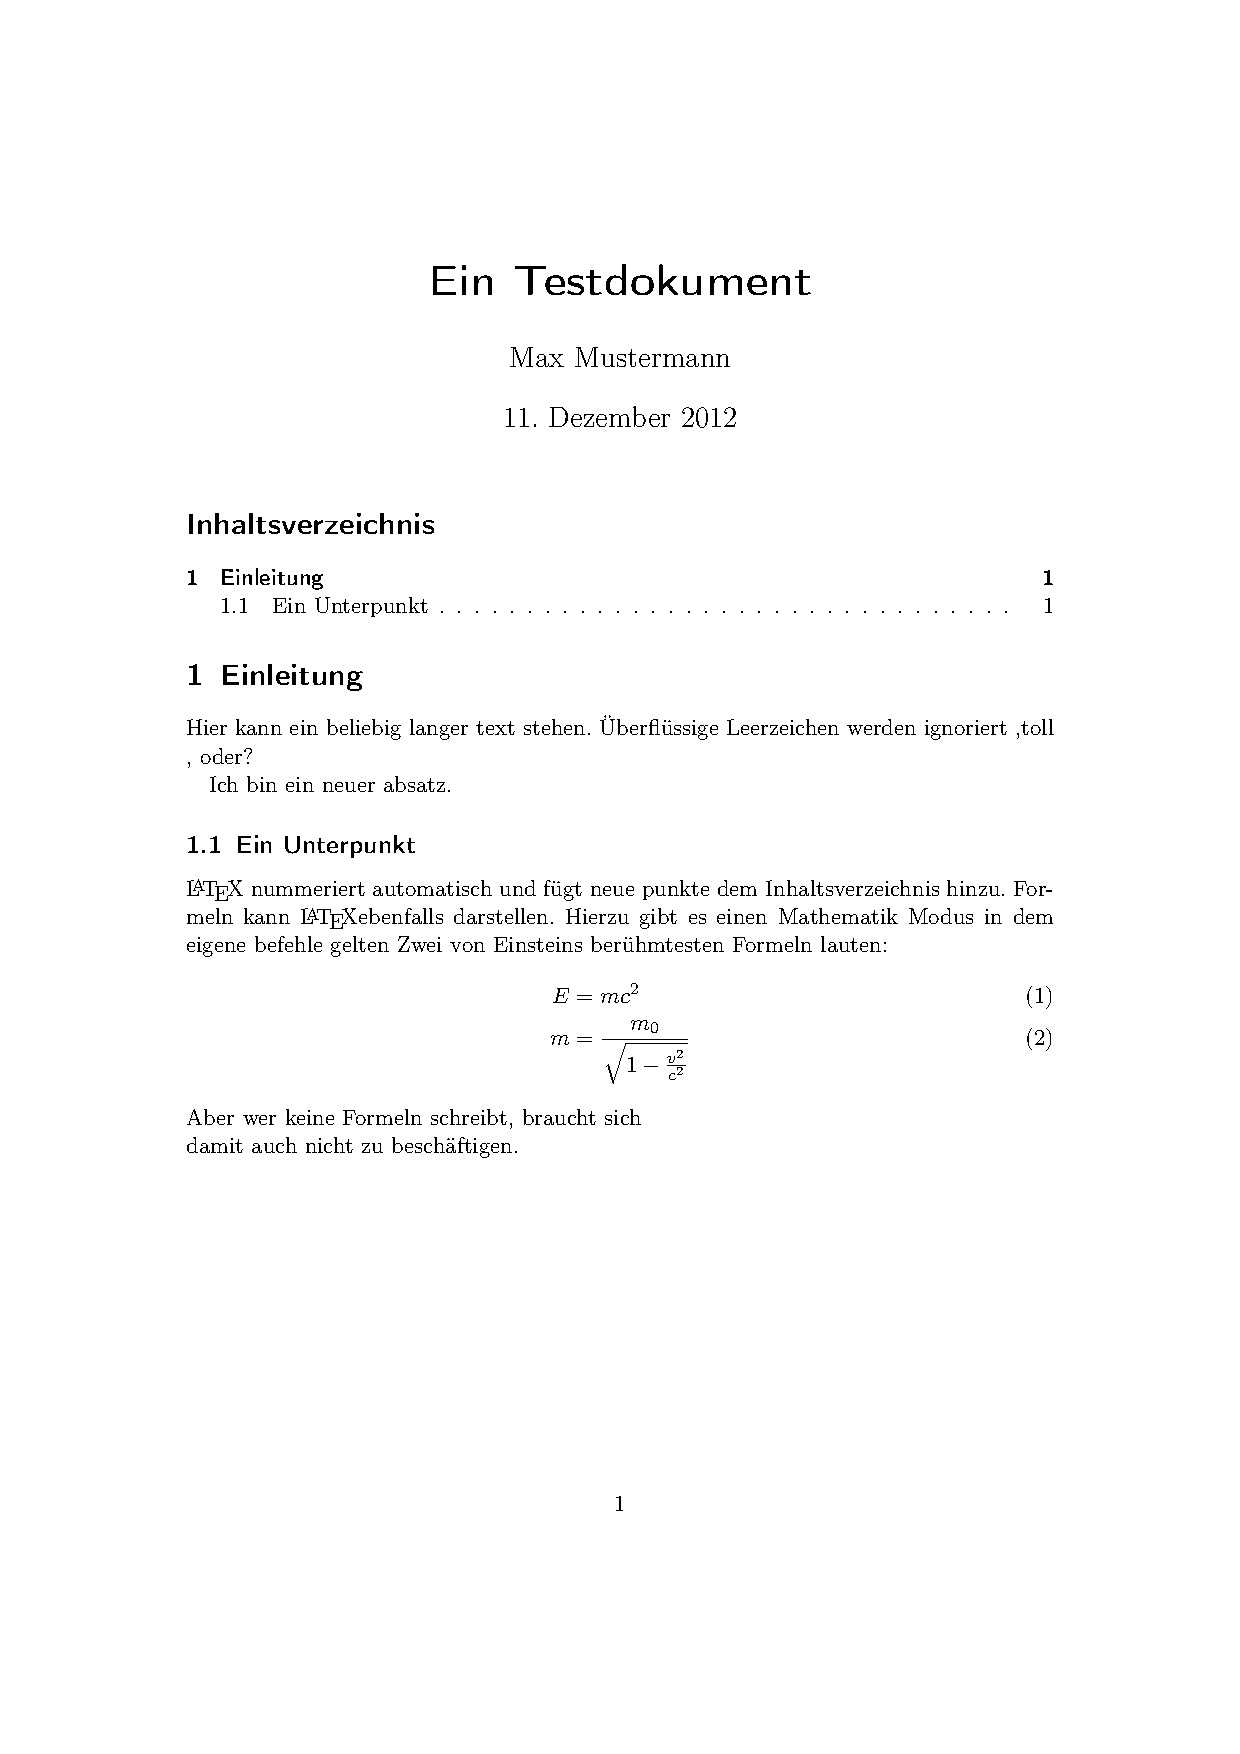
\includegraphics[height=\textheight]{./pictures/demonstration}
	\caption{Das PDF}
	\label{fig:demonstration}
	\end{figure}
\end{frame}

\begin{frame}{wichtige Befehle}
	\begin{itemize}[<+->]
	\item \lstinputlisting[linerange=1-1]{./listings/commands.tex} $ \Rightarrow $ \textbf{fett}
	\item \lstinputlisting[linerange=2-2]{./listings/commands.tex} $ \Rightarrow $ \textit{kursiv}
	\item \lstinputlisting[linerange=3-3]{./listings/commands.tex} $ \Rightarrow $ \underline{unterstrichen}
	\item \lstinputlisting[linerange=4-4]{./listings/commands.tex} $ \Rightarrow $ \textbf{\textit{\underline{kombination}}}
	\end{itemize}
\end{frame}
\section{Ansätze Office  vs  \LaTeX}
% \begin{frame}
 	\frametitle{Inhalt}
 	\tableofcontents[%
 		currentsection, % causes all sections but the current to be shown in a semi-transparent way.
% % 		currentsubsection, % causes all subsections but the current subsection in the current section to ...
% % 		hideallsubsections, % causes all subsections to be hidden.
% 		hideothersubsections, % causes the subsections of sections other than the current one to be hidden.
% % 		part=, % part number causes the table of contents of part part number to be shown
% 		pausesections, % causes a \pause command to be issued before each section. This is useful if you
% 		pausesubsections, %  causes a \pause command to be issued before each subsection.
% % 		sections={ overlay specification },
 	]
 \end{frame}
\begin{frame}{Ansätze Office  vs  \LaTeX}
	\begin{columns}
	
		 \column{0.45\textwidth}
		Office
		\begin{itemize}
			\item WYSIWYG
			\item volle Kontrolle des Nutzers über die Formatierung
			\item Anwender MUSS sich um alles selbst kümmern
			\item Arbeitsaufwand steigt mit Umfang des Dokuments
		\end{itemize}
		
		\column{0.45\textwidth}
		\LaTeX{}
		\begin{itemize}
				\item kein WYSIWYG
				\item Nutzer gibt absichtlich einen teil der Kontrolle ab
				\item Anwender kümmert sich nur um Format vorgaben
				\item Arbeitsaufwand sinkt, Autor kann sich auf das reine Schreiben konzentrieren
		\end{itemize}
	\end{columns}
\end{frame}
\begin{frame}{Arbeitsaufwand}
	\begin{figure}[htbp]
	\centering
		\begin{tikzpicture}[domain=0:5]
		
		  \draw[->,thick] (0,0)-- coordinate(x axis mid) (5.5,0) node[below] {Umfang des Dokuments };
		  \draw[->,thick] (0,0) -- coordinate(y axis mid) (0,4.5) node[left=0.5cm, rotate=90] {Arbeitsaufwand};
		  \draw[color=blue,domain=0.25:5] plot (\x,{ 1/ \x }) node[right] {\LaTeX};
		
		  \draw[color=orange,domain=0:4.5] plot (\x,{0.05*exp(\x)}) node[right] {Office};
		\end{tikzpicture}
	\end{figure}
\end{frame}
\begin{frame}{Wann nehme ich was?}
	\begin{columns}
	\centering
		\begin{column}{0.45\textwidth}
			Office
			\begin{itemize}[<+->]
			\item kleinere arbeiten 2-3
			\item Effektvolle Präsentationen
			\item wenn es schnell gehen muss und der Umfang gering ist
			\end{itemize}
		\end{column}
		\begin{column}{0.45\textwidth}
			\LaTeX
			\begin{itemize}[<+->]
			\item größere Arbeiten (Bachelor-,Master-,Diplomarbeit, Bücher)
			\item wenn mehrere Autoren beteiligt sind
			\item wenn ein Dokument Jahre später immer noch gleich aussehen soll
			\end{itemize}
		\end{column}
	\end{columns}
\end{frame}
\begin{frame}{Weitere Gründe für \LaTeX}
	\begin{figure}[tbph]
		\centering
		
\includegraphics[width=0.9\linewidth]{./pictures/hoeller1}
		\label{fig:hoeller1}
	\end{figure}
\end{frame}
\begin{frame}{Weitere Gründe für \LaTeX}
	\begin{figure}[tbph]
		\centering
		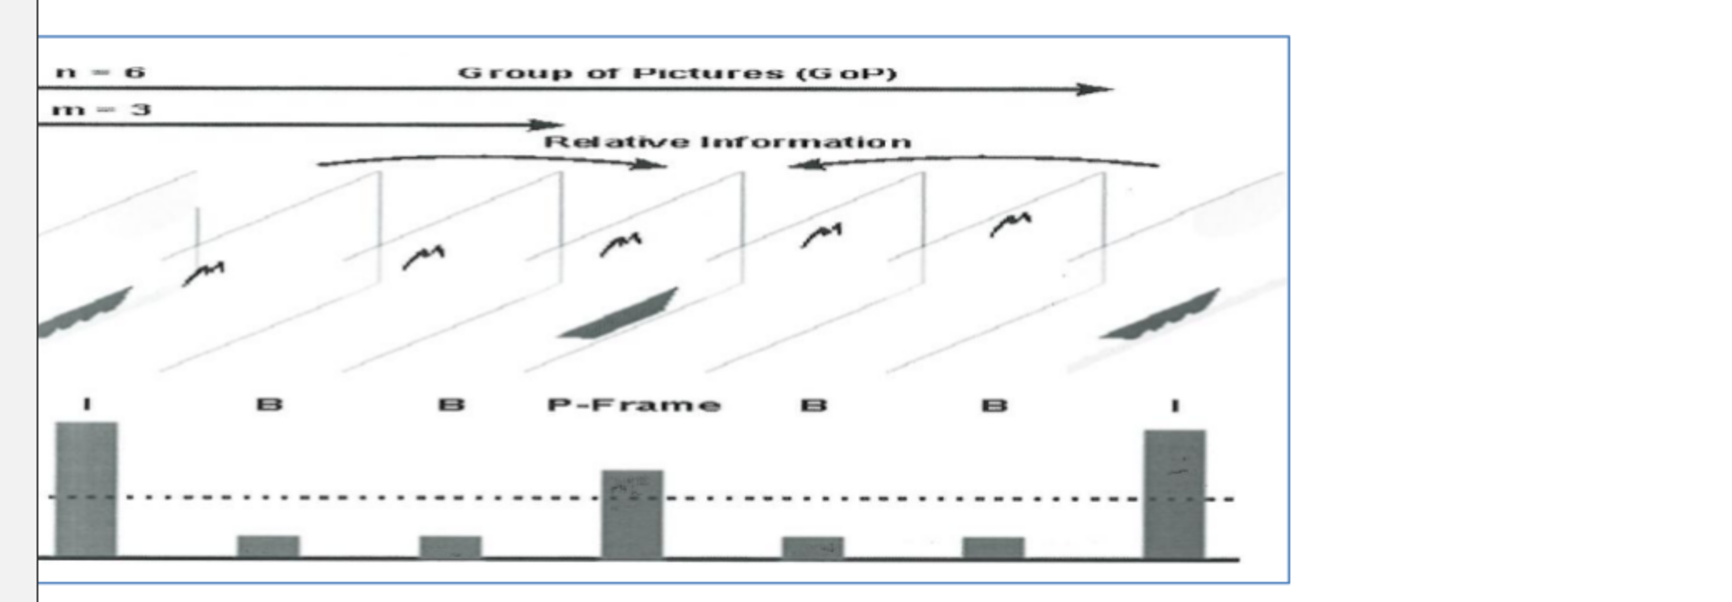
\includegraphics[width=0.9\linewidth]{./pictures/hoeller2}
		\label{fig:hoeller2}
	\end{figure}
\end{frame}
\begin{frame}{Weitere Gründe für \LaTeX}
\begin{figure}[tbph]
\centering
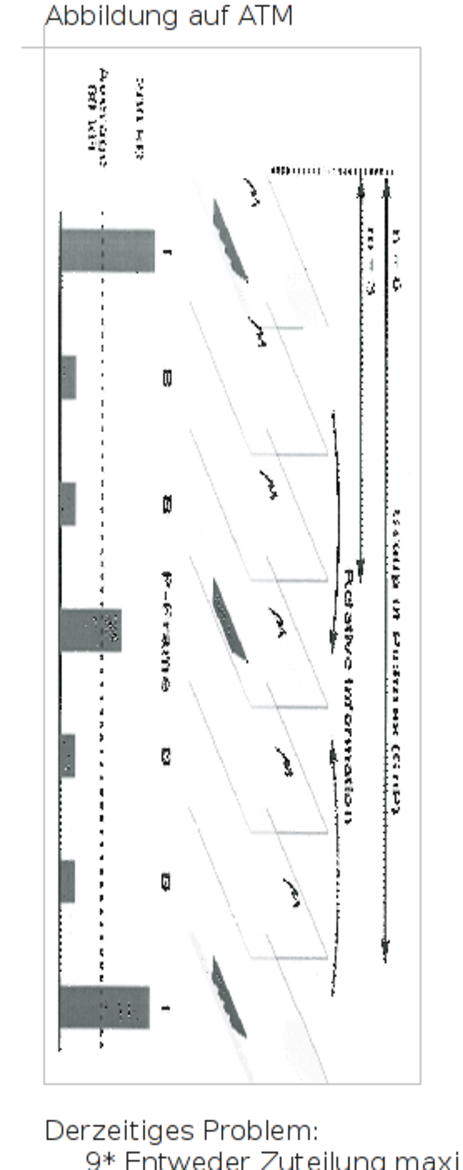
\includegraphics[height=0.75\textheight]{./pictures/hoeller3}
\label{fig:hoeller3}
\end{figure}
\end{frame}

\section{Editoren}
\begin{frame}{Editoren}
 \begin{itemize}[<+->]
 	\item AUCTeX
 	\item Eclipse (IDE) + TeXclipse
 	\item Geany
 	\item gedit
 	\item Kile
 	\item TeXstudio $ \leftarrow $ mein Favorit $\smiley$
 	\item \ldots
 \end{itemize}

\end{frame}
\section{Dokument Aufteilen \& Quellcodedarstellung}
\begin{frame}{Ein Dokument aufteilen}
\lstsettex
	\begin{Code}
	\centering
	\begin{minipage}{0.7\linewidth}
	\lstinputlisting[linerange=31-37]{./listings/commands.tex}
	\end{minipage}
	
	\end{Code}
\end{frame}
\begin{frame}{Quellcode}
	 benötigt wird das \textbf{listings} oder das \textbf{listingsutf8} package
\lstsettex
	\begin{Code}
	\centering
	\begin{minipage}{0.9\linewidth}
	\lstinputlisting[linerange=38-53,caption={Darstellung festlegen}]{./listings/commands.tex}
	\end{minipage}	
	\end{Code}
\end{frame}
\begin{frame}{Beispiel}
\lstsettex
	\begin{Code}
	\centering
	\begin{minipage}{0.9\linewidth}
	\lstinputlisting[linerange=54-62,caption={Quellcode einbinden}]{./listings/commands.tex}
	\end{minipage}	
	\end{Code}
\end{frame}

\begin{frame}{So sieht's im pdf aus}
\lstsetjava
\begin{Code}
	\centering
	\begin{minipage}{0.9\linewidth}
	\lstinputlisting[linerange=63-68,caption={This is Java}]{./listings/commands.tex}
	\end{minipage}	
	\end{Code}
\end{frame}
\section{Weitere Gründe \& Editoren}
\begin{frame}{Weitere Gründe für \LaTeX}
	\begin{figure}[tbph]
		\centering
		
\includegraphics[width=0.9\linewidth]{./pictures/hoeller1}
		\label{fig:hoeller1}
	\end{figure}
\end{frame}
\begin{frame}{Weitere Gründe für \LaTeX}
	\begin{figure}[tbph]
		\centering
		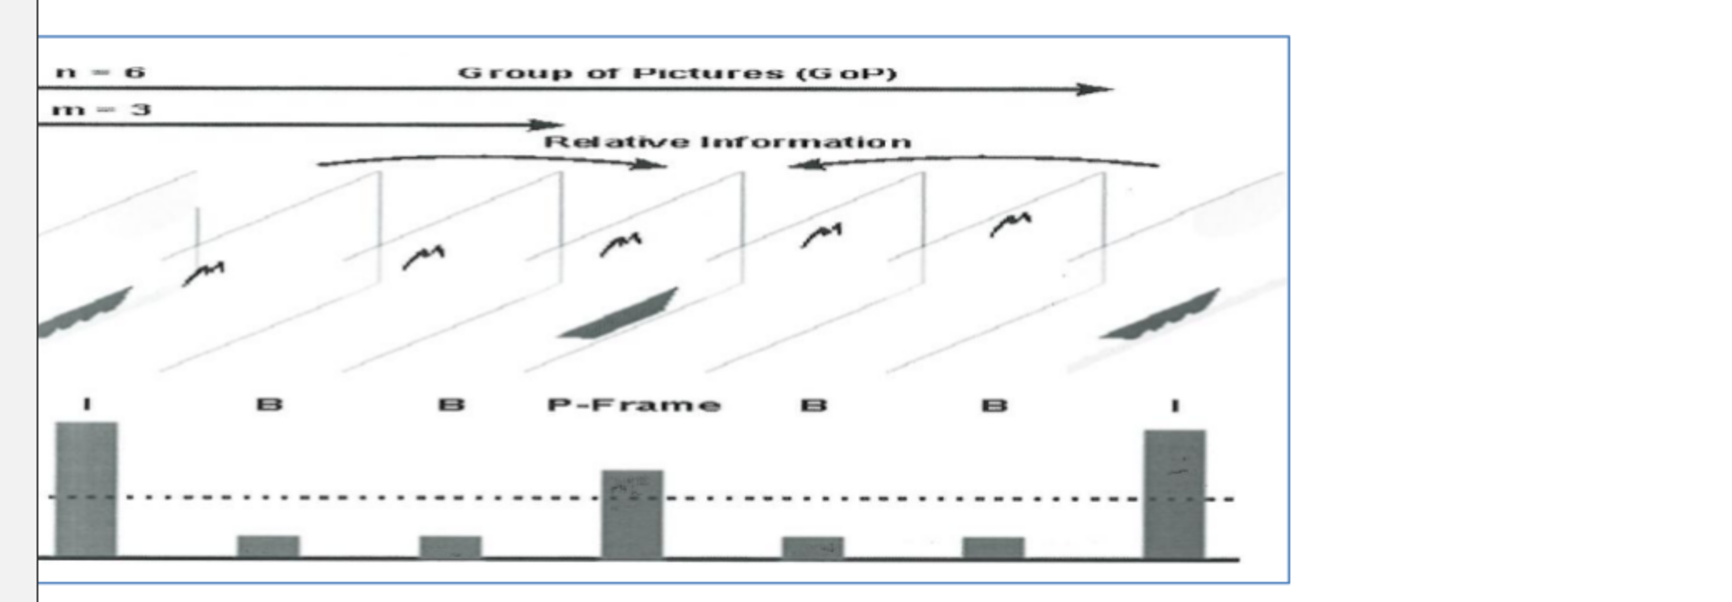
\includegraphics[width=0.9\linewidth]{./pictures/hoeller2}
		\label{fig:hoeller2}
	\end{figure}
\end{frame}
\begin{frame}{Weitere Gründe für \LaTeX}
\begin{figure}[tbph]
\centering
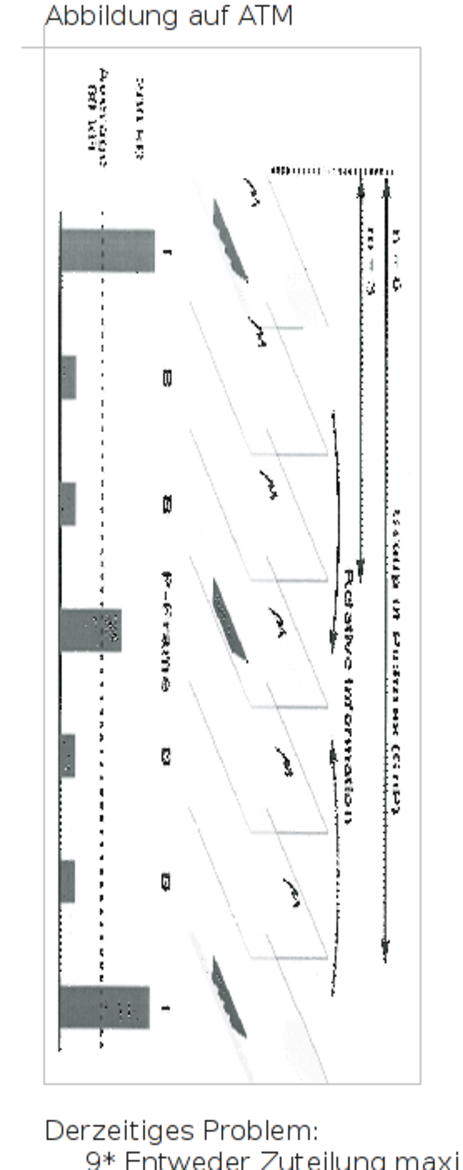
\includegraphics[height=0.75\textheight]{./pictures/hoeller3}
\label{fig:hoeller3}
\end{figure}
\end{frame}

\begin{frame}{Editoren}
 \begin{itemize}[<+->]
 	\item AUCTeX
 	\item Eclipse (IDE) + TeXclipse
 	\item Geany
 	\item gedit
 	\item Kile
 	\item TeXstudio $ \leftarrow $ mein Favorit $\smiley$
 	\item \ldots
 \end{itemize}

\end{frame}
\part{kai}
 \begin{frame}
 	\frametitle{Inhalt}
 	\tableofcontents[%
% 		currentsection, % causes all sections but the current to be shown in a semi-transparent way.
% % 		currentsubsection, % causes all subsections but the current subsection in the current section to ...
% % 		hideallsubsections, % causes all subsections to be hidden.
% 		hideothersubsections, % causes the subsections of sections other than the current one to be hidden.
% % 		part=, % part number causes the table of contents of part part number to be shown
 	%	pausesections, % causes a \pause command to be issued before each section. This is useful if you
% 		pausesubsections, %  causes a \pause command to be issued before each subsection.
% % 		sections={ overlay specification },
 ]
 \end{frame}
%hier gehts los

\section{TikZ}
\begin{frame}
\frametitle{Umgebung}
\begin{itemize}
  \item Zum Zeichnen unter \LaTeX wird nachfolgend TikZ verwendet
  \item die Zeichenumgebung wird mit $\backslash$ begin\{tikzpicture\} begonnen
\end{itemize}
\end{frame}

\begin{frame}
\frametitle{Kreise}
\begin{table}[!h]
\begin{tabular}{lr}

$\backslash$begin\{tikzpicture\} & \\
\\
$\backslash$path[draw] (0,0) circle (2ex) 
&
\begin{tikzpicture}
  \path[draw] (0,0) circle (2ex);
\end{tikzpicture} 
\\  
\\
$\backslash$path[fill] (0,-2) circle (2ex) 
&
\begin{tikzpicture}
  \path[fill] (0,0) circle (2ex);
\end{tikzpicture}
\\
\\
$\backslash$path[fill=yellow, draw=red] (0,-4) circle (2ex)
&
\begin{tikzpicture}
  \path[fill=yellow,draw=red] (0,0) circle (2ex);
\end{tikzpicture}
\\
\\
$\backslash$end\{tikzpicture\} & \\
\end{tabular}
\end{table}
\end{frame}

\begin{frame}
\frametitle{Diagramme}
\begin{figure}[!h]
\begin{tikzpicture}[domain=0:5]
  \draw[very thin,color=gray] (-0.1,-1.2) grid (4.9,3.2);
  \draw[->,thick] (-0.2,0) -- (5.5,0) node[right] {$x$};
  \draw[->,thick] (0,-1.2) -- (0,3.5) node[above] {$f(x)$};
  \draw[color=blue] plot (\x,{sin(\x r)}) node[right] {$f(x) = \sin x$};
  \draw[color=green] plot (\x,{cos(\x r)}) node[right] {$f(x) = \cos x$};
  \draw[color=orange,domain=0:4] plot (\x,{0.05*exp(\x)}) node[right] {$f(x) = \frac{1}{20} \mathrm e^x$};
\end{tikzpicture}


\end{figure}
\end{frame}

\begin{frame}
\frametitle{Diagramme}
	\lstsettex
	\lstinputlisting{./listings/diagram.tex}
\end{frame}

\begin{frame}
\frametitle{Graphen}
\begin{figure}[!h]
\begin{tikzpicture}
  \node (A) at (0, 4) [circle, fill=gray!30] {A};
  \node (B) at (3, 4) [circle, fill=gray!30] {B};
  \node (C) at (0, 2) [circle, fill=gray!30] {C};
  \node (D) at (3, 2) [circle, fill=gray!30] {D};
  \node (E) at (0, 0) [circle, fill=gray!30] {E};
  \node (F) at (3, 0) [circle, fill=gray!30] {F};

  \draw[->, very thick] (A) to (B);
  \draw[->, very thick] (B) to (D);
  \draw[->, very thick] (D) to (A);
  \draw[->, very thick] (A) to (C);
  \draw[->, very thick] (C) to (E);
  \draw[->, very thick] (E) to node[pos=0.3,above] {\tiny{Von E nach F}} (F);
  \draw[->, very thick] (F) to[loop above] (F);
\end{tikzpicture}

\end{figure}
\end{frame}

\begin{frame}
\frametitle{Graphen}
	\lstsettex
	\lstinputlisting{./listings/graph.tex}
\end{frame}

\begin{frame}
\frametitle{Feistel}
\begin{figure}[!h]
\begin{tikzpicture}[scale=1.1]
  \node [circle, fill=gray!30] (c1) at (0, 0) {$ 0001 $};
  \node [circle, fill=gray!30] (c2) at (5, 0) {$ 1111 $};
  \node (a1) at (0,1) [fill=gray!30] {$L(i+1)=l_1 (i+1), ... ,l_32(i+1)$};
  \node (a2) at (5,1) [fill=gray!30] {$R(i+1)=r_1 (i+1), ... ,r_32(i+1)$};
  \node (a3) at (0,4) [fill=gray!30] {$L(i)=l_1 , ... , l_32 (i)$};
  \node (a4) at (5,4) [fill=gray!30] {$R(i)=r_1 , ... , r_32 (i)$};
  \node [circle, fill=gray!30] (c3) at (0, 5) {$ 1101 $};
  \node [circle, fill=gray!30] (c4) at (5, 5) {$ 0001 $};
  \node [circle, fill=gray!30] (c5) at (0, 3) {$ + $};
  \node (a5) at (2.5,3) [fill=gray!30] {$f_i$};
  \node (a6) at (7,3) [fill=gray!30] {$K_i$};

  \draw[->, thick] (c3) to (a3);
  \draw[->, thick] (c4) to (a4);
  \draw[->, thick] (a3) to (c5);
  \draw[->, thick] (a1) to (c1);
  \draw[->, thick] (a2) to (c2);
  \draw[->, thick] (a6) to (a5);
  \draw[->, thick] (a5) to (c5);
  \draw[->, thick] (c5) to[out=-90, in=90] (a2)  ;
  \draw[->, thick] (a4) to[out=-90, in=90] (a1)  ;
  \draw[->, thick] (a4) to[out=-90, in=90] (a5)  ;
\end{tikzpicture}

\end{figure}
\end{frame}

\begin{frame}
\frametitle{Feistel}
	\lstsettex
	\lstinputlisting{./listings/feistel.tex}
\end{frame}


%   \title{beamer examples}
\subtitle{created with beamer 3.x}
\author{Matthias Pospiech}
\institute{University of Hannover}
\titlegraphic{}
\date{\today}
% --------------------------------------------------- Slide --
\begin{frame}[plain]
  \titlepage
\end{frame}
% --------------------------------------------------- Slide --
% \section[Contents]{}
% ------------------------------------------------------------
% \begin{frame}
% 	\frametitle{Contents}
% 	\tableofcontents[%
% 		currentsection, % causes all sections but the current to be shown in a semi-transparent way.
% % 		currentsubsection, % causes all subsections but the current subsection in the current section to ...
% % 		hideallsubsections, % causes all subsections to be hidden.
% 		hideothersubsections, % causes the subsections of sections other than the current one to be hidden.
% % 		part=, % part number causes the table of contents of part part number to be shown
% 		pausesections, % causes a \pause command to be issued before each section. This is useful if you
% % 		pausesubsections, %  causes a \pause command to be issued before each subsection.
% % 		sections={ overlay specification },
% 	]
% \end{frame}
% --------------------------------------------------- PART ---
\part{Tutorial}
\frame{\partpage}
% ------------------------------------------------------------
\begin{frame}
	\frametitle{Contents}
	\tableofcontents[%
% 		currentsection, % causes all sections but the current to be shown in a semi-transparent way.
% 		currentsubsection, % causes all subsections but the current subsection in the current section to ...
% 		hideallsubsections, % causes all subsections to be hidden.
% 		hideothersubsections, % causes the subsections of sections other than the current one to be hidden.
% 		part=, % part number causes the table of contents of part part number to be shown
		pausesections, % causes a \pause command to be issued before each section. This is useful if you
% 		pausesubsections, %  causes a \pause command to be issued before each subsection.
% 		sections={ overlay specification },
	]
\end{frame}
% ------------------------------------------------------------
\section{Tutorial: Euclid's Presentation}
% ------------------------------------------------------------
% --------------------------------------------------- Slide --
\subsection{Creating a Simple Frame}
% ------------------------------------------------------------
\begin{frame}
  \frametitle{What Are Prime Numbers?}
  A prime number is a number that has exactly two divisors.
\end{frame}
% --------------------------------------------------- Slide --
\begin{frame}
  \frametitle{What Are Prime Numbers?}
  \begin{definition}
    A \alert{prime number} is a number that has exactly two divisors
  \end{definition}
  \begin{example}
    \begin{itemize}
    \item 2 is prime (two divisors: 1 and 2).
    \item 3 is prime (two divisors: 1 and 3).
    \item 4 is not prime (\alert{three} divisors: 1, 2, and 4).
    \end{itemize}
  \end{example}
\end{frame}
% --------------------------------------------------- Slide --
\subsection{Creating Simple Overlays}
% ------------------------------------------------------------
\begin{frame}
  \frametitle{What Are Prime Numbers?}
  \begin{definition}
    A \alert{prime number} is a number that has exactly two divisors
  \end{definition}
  \begin{example}
		\begin{itemize}
			\item 2 is prime (two divisors: 1 and 2).
  			\pause
			\item 3 is prime (two divisors: 1 and 3).
  			\pause
			\item 4 is not prime (\alert{three} divisors: 1, 2, and 4).
		\end{itemize}
  \end{example}
\end{frame}
% --------------------------------------------------- Slide --
\begin{frame}
  \frametitle{There Is No Largest Prime Number}
  \framesubtitle{The proof uses \textit{reductio ad absurdum}.}
  \begin{theorem}
    There is no largest prime number.
  \end{theorem}
  \begin{proof}
    \begin{enumerate}
    \item<1-> Suppose $p$ were the largest prime number.
    \item<2-> Let $q$ be the product of the first $p$ numbers.
    \item<3-> Then $q + 1$ is not divisible by any of them.
    \item<1-> Thus $q + 1$ is also prime and greater than $p$.\qedhere
    \end{enumerate}
  \end{proof}
  \uncover<4->{The proof used \textit{reductio ad absurdum}.}
\end{frame}
% --------------------------------------------------- Slide --
\subsection{Structuring a Frame}
% ------------------------------------------------------------
\newtheorem{answeredquestions}[theorem]{Answered Questions}
\newtheorem{openquestions}[theorem]{Open Questions}
% ------------------------------------------------------------
\begin{frame}
  \frametitle{What's Still To Do?}
  \begin{block}{Answered Questions}
    How many primes are there?
  \end{block}
  \begin{block}{Open Questions}
    Is every even number the sum of two primes?
  \end{block}
\end{frame}
% --------------------------------------------------- Slide --
\begin{frame}
  \frametitle{What's Still To Do?}
  \begin{itemize}
  \item Answered Questions
    \begin{itemize}
    \item How many primes are there?
    \end{itemize}
  \item Open Questions
    \begin{itemize}
    \item Is every even number the sum of two primes?
    \end{itemize}
  \end{itemize}
\end{frame}
% --------------------------------------------------- Slide --
\begin{frame}
  \frametitle{What's Still To Do?}
  \begin{columns}
    \column{.5\textwidth}
      \begin{block}{Answered Questions}
        How many primes are there?
      \end{block}
    \column{.5\textwidth}
      \begin{block}{Open Questions}
        Is every even number the sum of two primes?
        \cite{Goldbach1742}
      \end{block}
  \end{columns}
\end{frame}
% --------------------------------------------------- Slide --
\subsection{Verbatim Text}
% ------------------------------------------------------------
\begin{frame}[fragile]
  \frametitle{An Algorithm For Finding Primes Numbers.}
	\begin{verbatim}
int main (void)
{
  std::vector<bool> is_prime (100, true);
  for (int i = 2; i < 100; i++)
    if (is_prime[i])
      {
        std::cout << i << " ";
        for (int j = i; j < 100;
            is_prime [j] = false, j+=i);
      }
  return 0;
}
	\end{verbatim}
%  \begin{uncoverenv}<2>
%     Note the use of \verb|std::|.
%  \end{uncoverenv}
\end{frame}
% --------------------------------------------------- Slide --
\begin{frame}[fragile]
  \frametitle{An Algorithm For Finding Primes Numbers.}
\begin{semiverbatim}
\uncover<1->{\alert<0>{int main (void)}}
\uncover<1->{\alert<0>{\{}}
\uncover<1->{\alert<1>{ \alert<4>{std::}vector<bool> is_prime (100, true);}}
\uncover<1->{\alert<1>{ for (int i = 2; i < 100; i++)}}
\uncover<2->{\alert<2>{    if (is_prime[i])}}
\uncover<2->{\alert<0>{      \{}}
\uncover<3->{\alert<3>{        \alert<4>{std::}cout << i << " ";}}
\uncover<3->{\alert<3>{        for (int j = i; j < 100;}}
\uncover<3->{\alert<3>{             is_prime [j] = false, j+=i);}}
\uncover<2->{\alert<0>{      \}}}
\uncover<1->{\alert<0>{ return 0;}}
\uncover<1->{\alert<0>{\}}}
\end{semiverbatim}
  \visible<4->{Note the use of \alert{\texttt{std::}}.}
\end{frame}
% --------------------------------------------------- PART ---
\part{Howtos}
\frame{\partpage}
% ------------------------------------------------------------
\begin{frame}
	\frametitle{Contents}
	\tableofcontents[%
% 		currentsection, % causes all sections but the current to be shown in a semi-transparent way.
% 		currentsubsection, % causes all subsections but the current subsection in the current section to ...
% 		hideallsubsections, % causes all subsections to be hidden.
% 		hideothersubsections, % causes the subsections of sections other than the current one to be hidden.
% 		part=, % part number causes the table of contents of part part number to be shown
		pausesections, % causes a \pause command to be issued before each section. This is useful if you
% 		pausesubsections, %  causes a \pause command to be issued before each subsection.
% 		sections={ overlay specification },
	]
\end{frame}
% ------------------------------------------------------------
\section{How To Uncover Things Piecewise}
% ------------------------------------------------------------
\subsection{Uncovering an Enumeration Piecewise}
% ------------------------------------------------------------
\begin{frame}
\begin{itemize}
\item<1-> First point.
\item<2-> Second point.
\item<3-> Third point.
\end{itemize}

\begin{itemize}[<+->]
\item First point.
\item Second point.
\item Third point.
\end{itemize}

\begin{itemize}[<+->]
\item First point.
\item<.-> Second point.
\item Third point.
\end{itemize}
\end{frame}
% --------------------------------------------------- Slide --
\subsection{Hilighting the Current Item in an Enumeration}
% ------------------------------------------------------------
\begin{frame}
\begin{itemize}
\item<1-| alert@1> First point.
\item<2-| alert@2> Second point.
\item<3-| alert@3> Third point.
\end{itemize}
or
\begin{itemize}[<+-| alert@+>]
\item First point.
\item Second point.
\item Third point.
\end{itemize}
\end{frame}
% --------------------------------------------------- Slide --
\subsection{Changing Symbol Before an Enumeration}
% ------------------------------------------------------------
\newenvironment{ballotenv}
{\only{%
  \setbeamertemplate{itemize item}{code for showing a ballot}%
  \setbeamertemplate{itemize subitem}{code for showing a smaller ballot}%
  \setbeamertemplate{itemize subsubitem}{code for showing a smaller ballot}}}
{}
\begin{frame}
\begin{itemize}
\item<1-| ballot@1> First point.
\item<2-| ballot@2> Second point.
\item<3-| ballot@3> Third point.
\end{itemize}
and
\begin{itemize}[<+-| ballot@+>]
\item First point.
\item Second point.
\item Third point.
\end{itemize}
\end{frame}
% --------------------------------------------------- Slide --
\begin{frame}
In the following example, more and more items become "checked" from slide to slide:
\begin{itemize}[<ballot@+-| visible@1-,+(1)>]
\item First point.
\item Second point.
\item Third point.
\end{itemize}
\end{frame}
% --------------------------------------------------- Slide --
\subsection{Uncovering Piecewise}
% ------------------------------------------------------------
\begin{frame}
Uncovering Tagged Formulas Piecewise
\begin{align}
  A &= B \\
    \uncover<2->{&= C \\}
    \uncover<3->{&= D \\}
    \notag
  \end{align}
\vskip-1.5em
\end{frame}

\begin{frame}
Uncovering a Table Rowwise \newline
\rowcolors[]{1}{blue!20}{blue!10}
\begin{tabular}{l!{\vrule}cccc}
  Class & A & B & C & D \\\hline
  X     & 1 & 2 & 3 & 4 \pause\\
  Y     & 3 & 4 & 5 & 6 \pause\\
  Z     &5&6&7&8
\end{tabular}
\end{frame}

\begin{frame}
Uncovering a Table Columnwise \newline
\rowcolors[]{1}{blue!20}{blue!10}
\begin{tabular}{l!{\vrule}c<{\onslide<2->}c<{\onslide<3->}c<{\onslide<4->}c<{\onslide}c}
  Class & A & B & C & D \\
  X     & 1 & 2 & 3 & 4 \\
  Y     & 3 & 4 & 5 & 6 \\
  Z     &5&6&7&8
\end{tabular}
\end{frame}
% --------------------------------------------------- PART ---
\part{Building a Presentation}
\frame{\partpage}
% ------------------------------------------------------------
\begin{frame}
	\frametitle{Contents}
	\tableofcontents[%
%   	currentsection, % causes all sections but the current to be shown in a semi-transparent way.
% 		currentsubsection, % causes all subsections but the current subsection in the current section to ...
 		hideallsubsections, % causes all subsections to be hidden.
% 		hideothersubsections, % causes the subsections of sections other than the current one to be hidden.
% 		part=, % part number causes the table of contents of part part number to be shown
		pausesections, % causes a \pause command to be issued before each section. This is useful if you
% 		pausesubsections, %  causes a \pause command to be issued before each subsection.
% 		sections={ overlay specification },
	]
\end{frame}
% --------------------------------------------------- Slide --
\section{Creating Overlays}
% ------------------------------------------------------------
\subsection{The Pause Commands}
% ------------------------------------------------------------
\begin{frame}
  \begin{itemize}
  \item
    Shown from first slide on.
  \pause
  \item
    Shown from second slide on.
    \begin{itemize}
    \item
      Shown from second slide on.
    \pause
    \item
      Shown from third slide on.
    \end{itemize}
  \item
    Shown from third slide on.
  \pause
  \item
    Shown from fourth slide on.
  \end{itemize}
  Shown from fourth slide on.
  \begin{itemize}
  \onslide
  \item
    Shown from first slide on.
  \pause
  \item
    Shown from fifth slide on.
  \end{itemize}
\end{frame}
% --------------------------------------------------- Slide --
\subsection{Commands with Overlay Specifications}
% ------------------------------------------------------------
\begin{frame}
  \textbf{This line is bold on all three slides.}
  \textbf<2>{This line is bold only on the second slide.}
  \textbf<3>{This line is bold only on the third slide.}
\end{frame}
% --------------------------------------------------- Slide --
\begin{frame}
  \only<1>{This line is inserted only on slide 1.}
  \only<2>{This line is inserted only on slide 2.}
\end{frame}
% --------------------------------------------------- Slide --
\begin{frame}
  Shown on first slide.
  \onslide<2-3>
  Shown on second and third slide.
  \begin{itemize}
  \item
    Still shown on the second and third slide.
  \onslide+<4->
  \item
    Shown from slide 4 on.
  \end{itemize}
  Shown from slide 4 on.
  \onslide
  Shown on all slides.
\end{frame}
% --------------------------------------------------- Slide --
\begin{frame}
  \onslide<1>{Same effect as the following command.}
  \uncover<1>{Same effect as the previous command.}
  \onslide+<2>{Same effect as the following command.}
  \visible<2>{Same effect as the previous command.}
  \onslide*<3>{Same effect as the following command.}
  \only<3>{Same effect as the previous command.}
\end{frame}
% --------------------------------------------------- Slide --
\begin{frame}
\temporal<3-4>{Shown on 1, 2}{Shown on 3, 4}{Shown 5, 6, 7, ...}
\temporal<3,5>{Shown on 1, 2, 4}{Shown on 3, 5}{Shown 6, 7, 8, ...}
\end{frame}
% --------------------------------------------------- Slide --
\def\colorize<#1>{%
  \temporal<#1>{\color{red!50}}{\color{black}}{\color{black!50}}}
\begin{frame}
  \begin{itemize}
    \colorize<1> \item First item.
    \colorize<2> \item Second item.
    \colorize<3> \item Third item.
    \colorize<4> \item Fourth item.
  \end{itemize}
\end{frame}
% --------------------------------------------------- Slide --
\begin{frame}
  \begin{enumerate}
  \item<3-| alert@3>[0.] A zeroth point, shown at the very end.
  \item<1-| alert@1> The first and main point.
  \item<2-| alert@2> The second point.
  \end{enumerate}
\end{frame}
% --------------------------------------------------- Slide --
\subsection{Environments with Overlay Specifications}
% ------------------------------------------------------------
\begin{frame}
  \frametitle{A Theorem on Infinite Sets}
  \begin{theorem}<1->
    There exists an infinite set.
  \end{theorem}
  \begin{proof}<3->
    This follows from the axiom of infinity.
  \end{proof}
  \begin{example}<2->
    The set of natural numbers is infinite.
  \end{example}
\end{frame}
% --------------------------------------------------- Slide --
\begin{frame}
  This line is always shown.
  \begin{onlyenv}<2>
    This line is inserted on slide 2.
  \end{onlyenv}
\end{frame}
% --------------------------------------------------- Slide --
\begin{frame}
  This
  \begin{altenv}<2>{(}{)}{[}{]}
    word
  \end{altenv}
  is in round brackets on slide 2 and in square brackets on slide 1.
\end{frame}
% --------------------------------------------------- Slide --
\subsection{Dynamically Changing Text or Images}
% ------------------------------------------------------------
\begin{frame}
	\begin{overlayarea}{\textwidth}{3cm}
  		\only<1>{Some text for the first slide.\\ Possibly several lines long.}
  		\only<2>{Replacement on the second slide.}
	\end{overlayarea}
\end{frame}
% --------------------------------------------------- Slide --
\begin{frame}
	\begin{overprint}
  		\onslide<1| handout:1>
    		Some text for the first slide.\\
    		Possibly several lines long.
  		\onslide<2| handout:0>
    		Replacement on the second slide. Supressed for handout.
	\end{overprint}
\end{frame}
% --------------------------------------------------- Slide --
\subsection{Advanced Overlay Specifications}
% ------------------------------------------------------------
\begin{frame}
  \begin{actionenv}<1-| alert@3-4,6>
    This text is shown the same way as the text below.
  \end{actionenv}
  \begin{uncoverenv}<2->
    \begin{alertenv}<3-4,6>
      This text is shown the same way as the text above.
    \end{alertenv}
  \end{uncoverenv}
\end{frame}
% --------------------------------------------------- Slide --
\begin{frame}
	\begin{itemize}
		\item<+-> Apple
		\item<+-> Peach
		\item<+-> Plum
		\item<+-> Orange
	\end{itemize}

	\begin{itemize}[<+-| alert@+>]
		\item Apple
		\item Peach
		\item Plum
		\item Orange
	\end{itemize}

	\begin{itemize}[<+->]
		\item This is \alert<.>{important}.
		\item We want to \alert<.>{highlight} this and \alert<.>{this}.
		\item What is the \alert<.>{matrix}?
	\end{itemize}
\end{frame}
% --------------------------------------------------- Slide --
% \section{Adding Parts}
% % ------------------------------------------------------------
% \frame{\titlepage}
% \section*{Outlines}
% \subsection{Part I: Review of Previous Lecture}
% \frame{
%   \frametitle{Outline of Part I}
%   \tableofcontents[part=1]}
% \subsection{Part II: Today's Lecture}
% \frame{
%   \frametitle{Outline of Part II}
%   \tableofcontents[part=2]}
% \part{Review of Previous Lecture}
% \frame{\partpage}
% \section[Previous Lecture]{Summary of the Previous Lecture}
% \subsection{Topics}
% \frame{...}
% \subsection{Learning Objectives}
% \frame{...}
% \part{Today's Lecture}
% \frame{\partpage}
% \section{Topic A}
% \frame{\tableofcontents[currentsection]}
% \subsection{Foo}
% \frame{...}
% \section{Topic B}
% \frame{\tableofcontents[currentsection]}
% \subsection{bar}
% \frame{...}
% --------------------------------------------------- Slide --
\section{Structuring a Presentation: The Interactive Global Structure}
% ------------------------------------------------------------
\subsection{Adding Hyperlinks and Buttons}
% ------------------------------------------------------------
\begin{frame}
  \begin{itemize}
  \item<1-> First item.
  \item<2-> Second item.
  \item<3-> Third item.
  \end{itemize}
  \hyperlink{jumptosecond}{\beamergotobutton{Jump to second slide}}
  \hypertarget<2>{jumptosecond}{}
\end{frame}
% --------------------------------------------------- Slide --
\begin{frame}[label=threeitems]
  \begin{itemize}
  \item<1-> First item.
  \item<2-> Second item.
  \item<3-> Third item.
  \end{itemize}
  \hyperlink{threeitems<2>}{\beamergotobutton{Jump to second slide}}
\end{frame}
% --------------------------------------------------- Slide --
\frame{
  \begin{theorem}
    ...
  \end{theorem}
  \begin{overprint}
  \onslide<1>
    \hfill\hyperlinkframestartnext{\beamerskipbutton{Skip proof}}
  \onslide<2>
    \begin{proof}
      ...
    \end{proof}
  \end{overprint}
}
% --------------------------------------------------- Slide --
% \frame<1>[label=mytheorem]
% {
%   \begin{theorem}
%     ...
%   \end{theorem}
%   \begin{overprint}
%   \onslide<1>
%     \hfill\hyperlink{mytheorem<2>}{\beamergotobutton{Go to proof details}}
%   \onslide<2>
%     \begin{proof}
%       ...
%     \end{proof}
%     \hfill\hyperlink{mytheorem<1>}{\beamerreturnbutton{Return}}
%   \end{overprint}
% }
% \appendix
% \againframe<2>{mytheorem}
% % --------------------------------------------------- Slide --
% \subsection{Repeating a Frame at a Later Point}
% % ------------------------------------------------------------
% \frame<1-2>[label=myframe]
% {
%   \begin{itemize}
%   \item<alert@1> First subject.
%   \item<alert@2> Second subject.
%   \item<alert@3> Third subject.
%   \end{itemize}
% }
% \frame
% {
%   Some stuff explaining more on the second matter.
% }
% \againframe<3>{myframe}
% --------------------------------------------------- Slide --
% \subsection{Adding Anticipated Zooming}
% % ------------------------------------------------------------
% \begin{frame}<1>[label=zooms]
%   \frametitle<1>{A Complicated Picture}
%   \framezoom<1><2>[border](0cm,0cm)(2cm,1.5cm)
%   \framezoom<1><3>[border](1cm,3cm)(2cm,1.5cm)
%   \framezoom<1><4>[border](3cm,2cm)(3cm,2cm)
%   \pgfimage[height=8cm]{complicatedimagefilename}
% \end{frame}
% \againframe<2->[plain]{zooms}
% --------------------------------------------------- Slide --
\section{Structuring a Presentation: The Local Structure}
% ------------------------------------------------------------
\subsection{Itemizations, Enumerations, and Descriptions}
% ------------------------------------------------------------
\begin{frame}
  There are three important points:
  \begin{enumerate}
  \item<1-> A first one,
  \item<2-> a second one with a bunch of subpoints,
    \begin{itemize}
    \item first subpoint. (Only shown from second slide on!).
    \item<3-> second subpoint added on third slide.
    \item<4-> third subpoint added on fourth slide.
    \end{itemize}
  \item<5-> and a third one.
  \end{enumerate}
\end{frame}
% --------------------------------------------------- Slide --
\begin{frame}
\begin{itemize}[<+->]
\item This is shown from the first slide on.
\item This is shown from the second slide on.
\item This is shown from the third slide on.
\item<1-> This is shown from the first slide on.
\item This is shown from the fourth slide on.
\end{itemize}
\end{frame}
% --------------------------------------------------- Slide --
\begin{frame}
\begin{description}[<+->][longest label]
\item[short] Some text.
\item[longest label] Some text.
\item[long label] Some text.
\end{description}
\end{frame}
% --------------------------------------------------- Slide --
\subsection{Block Environments}
% ------------------------------------------------------------
\begin{frame}
	\begin{block}<1->{Definition}
  		A \alert{set} consists of elements.
	\end{block}
	\begin{alertblock}{Wrong Theorem}
  		$1=2$.
	\end{alertblock}
	\begin{exampleblock}{Example}<only@2->
  		The set $\{1,2,3,5\}$ has four elements.
	\end{exampleblock}
\end{frame}
% --------------------------------------------------- Slide --
\subsection{Theorem Environments}
% ------------------------------------------------------------
\begin{frame}
  \frametitle{A Theorem on Infinite Sets}
  \begin{theorem}<1->
    There exists an infinite set.
  \end{theorem}
  \begin{proof}<2->
    This follows from the axiom of infinity.
  \end{proof}
  \begin{example}<3->[Natural Numbers]
    The set of natural numbers is infinite.
  \end{example}
\end{frame}
% --------------------------------------------------- Slide --
\subsection{Framed and Boxed Text}
% ------------------------------------------------------------
\begin{frame}
	\begin{beamercolorbox}[ht=2.5ex,dp=1ex,center]{title in head/foot}
  		\usebeamerfont{title in head/foot}
  		\insertshorttitle
	\end{beamercolorbox}%
	\begin{beamercolorbox}[ht=2.5ex,dp=1ex,center]{author in head/foot}
  		\usebeamerfont{author in head/foot}
  		\insertshortauthor
	\end{beamercolorbox}
	\mbox{}\medskip\newline
	Typesetting a postit:\newline
	\setbeamercolor{postit}{fg=black,bg=yellow}
	\begin{beamercolorbox}[sep=1em,wd=5cm]{postit}
  		Place me somewhere!
	\end{beamercolorbox}
	\mbox{}\medskip\newline
	\begin{beamerboxesrounded}[upper=block head,lower=block body,shadow=true]{Theorem}
  		$A = B$.
	\end{beamerboxesrounded}
\end{frame}
% --------------------------------------------------- Slide --
\subsection{Splitting a Frame into Multiple Columns}
% ------------------------------------------------------------
\begin{frame}
	\begin{columns}[t]
  		\begin{column}{5cm}
    		Two\\lines.
  		\end{column}
  		\begin{column}{5cm}
    		One line (but aligned).
  		\end{column}
	\end{columns}
\end{frame}
% --------------------------------------------------- Slide --
\section{Animations, Sounds, and Slide Transitions}
% ------------------------------------------------------------
\subsection{Animations Created by Showing Slides in Rapid Succession}
% ------------------------------------------------------------
% \begin{frame}
%   \frametitle{A Five Slide Animation}
%   \animate<2-4>
%   ... code for creating an animation with five slides ...
% \end{frame}
% --------------------------------------------------- Slide --
\newcount\opaqueness
\begin{frame}
  anomations only work in full screen mode in Acrobat Reader !
  \animate<2-10>
  \animatevalue<1-10>{\opaqueness}{100}{0}
  \begin{colormixin}{\the\opaqueness!averagebackgroundcolor}
    \frametitle{Fadeout Frame}
    This text (and all other frame content) will fade out when the
    second slide is shown. This even works with
    {\color{green!90!black}colored} \alert{text}.
  \end{colormixin}
\end{frame}
\newcount\opaqueness
\newdimen\offset
\begin{frame}
  \frametitle{Flying Theorems (You Really Shouldn't!)}
  \animate<2-14>
  \animatevalue<1-15>{\opaqueness}{100}{0}
  \animatevalue<1-15>{\offset}{0cm}{-5cm}
  \begin{colormixin}{\the\opaqueness!averagebackgroundcolor}
  \hskip\offset
    \begin{minipage}{\textwidth}
      \begin{theorem}
        This theorem flies out.
      \end{theorem}
    \end{minipage}
  \end{colormixin}
  \animatevalue<1-15>{\opaqueness}{0}{100}
  \animatevalue<1-15>{\offset}{-5cm}{0cm}
  \begin{colormixin}{\the\opaqueness!averagebackgroundcolor}
  \hskip\offset
    \begin{minipage}{\textwidth}
      \begin{theorem}
        This theorem flies in.
      \end{theorem}
    \end{minipage}
  \end{colormixin}
\end{frame}
% --------------------------------------------------- Slide --
\subsection{Slide Transitions}
% ------------------------------------------------------------
\begin{frame}
	Slide Transitions only work in full screen mode in Acrobat Reader !
  \begin{example}<1,6,11>[examples for Slide Transitions]{This line is shown on each slide of slide transitions}\end{example}
  \begin{example}<2,7,12>[examples for Slide Transitions]{This line is shown on each slide of slide transitions}\end{example}
  \begin{example}<3,8>[examples for Slide Transitions]{This line is shown on each slide of slide transitions}\end{example}
  \begin{example}<4,9>[examples for Slide Transitions]{This line is shown on each slide of slide transitions}\end{example}
  \begin{example}<5,10>[examples for Slide Transitions]{This line is shown on each slide of slide transitions}\end{example}
  \transdissolve<1>[duration=0.2]
  \transblindshorizontal<2>
  \transblindsvertical<3>
  \transboxin<4>
  \transboxout<5>
  \transdissolve<6>[duration=0.2]
  \transglitter<7>[direction=90]
  \transsplitverticalin<8>
  \transsplitverticalout<9>
  \transsplithorizontalin<10>
  \transsplithorizontalout<11>
  \transwipe<12>[direction=90]
\end{frame}

% --------------------------------------------------- Slide --
\section{Adding Notes}
% ------------------------------------------------------------
\begin{frame}
  \begin{itemize}
  \item<1-> Eggs
  \item<2-> Plants
    \note[item]<2>{Tell joke about plants.}
    \note[item]<2>{Make it short.}
  \item<3-> Animals
  \end{itemize}
\end{frame}

% % --------------------------------------------------- Slide --
% \begin{frame}
%
% \end{frame}

% ------------------------------------------------------------
\begin{thebibliography}{10}
\bibitem{Goldbach1742}[Goldbach, 1742]
  Christian Goldbach.
  \newblock A problem we should try to solve before the ISPN '43 deadline,
  \newblock \emph{Letter to Leonhard Euler}, 1742.
\end{thebibliography}

%  	\input{content/Beamer-Title}
%  	\input{content/Beamer-Content}
%  	\input{content/Beamer-Appendix}
\end{document}
